\mbox{$\displaystyle $\,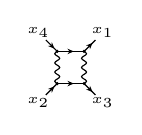
\begin{tikzpicture}[x=0.340cm, y=0.340cm, line width=0.420pt, baseline={([yshift=-0.6ex]0,0)}]
  \draw (-0.500,0.600) -- (0.500,0.600);
  \fill (0.119,0.600) -- (-0.119,0.702) -- (-0.042,0.600) -- (-0.119,0.498) -- cycle;
  \draw (-0.500,-0.600) -- (0.500,-0.600);
  \fill (0.119,-0.600) -- (-0.119,-0.498) -- (-0.042,-0.600) -- (-0.119,-0.702) -- cycle;
  \draw plot[smooth, tension=0.7] coordinates {(0.500,0.600) (0.565,0.557) (0.593,0.514) (0.565,0.471) (0.500,0.429) (0.435,0.386) (0.407,0.343) (0.435,0.300) (0.500,0.257) (0.565,0.214) (0.593,0.171) (0.565,0.129) (0.500,0.086) (0.435,0.043) (0.407,0.000) (0.435,-0.043) (0.500,-0.086) (0.565,-0.129) (0.593,-0.171) (0.565,-0.214) (0.500,-0.257) (0.435,-0.300) (0.407,-0.343) (0.435,-0.386) (0.500,-0.429) (0.565,-0.471) (0.593,-0.514) (0.565,-0.557) (0.500,-0.600)};
  \draw plot[smooth, tension=0.7] coordinates {(-0.500,-0.600) (-0.565,-0.557) (-0.593,-0.514) (-0.565,-0.471) (-0.500,-0.429) (-0.435,-0.386) (-0.407,-0.343) (-0.435,-0.300) (-0.500,-0.257) (-0.565,-0.214) (-0.593,-0.171) (-0.565,-0.129) (-0.500,-0.086) (-0.435,-0.043) (-0.407,0.000) (-0.435,0.043) (-0.500,0.086) (-0.565,0.129) (-0.593,0.171) (-0.565,0.214) (-0.500,0.257) (-0.435,0.300) (-0.407,0.343) (-0.435,0.386) (-0.500,0.429) (-0.565,0.471) (-0.593,0.514) (-0.565,0.557) (-0.500,0.600)};
  \draw (0.500,0.600) -- (0.924,1.024);
  \fill (0.818,0.918) -- (0.577,0.821) -- (0.704,0.804) -- (0.721,0.677) -- cycle;
  \draw (-0.500,-0.600) -- (-0.924,-1.024);
  \fill (-0.606,-0.706) -- (-0.847,-0.803) -- (-0.720,-0.820) -- (-0.703,-0.947) -- cycle;
  \draw (0.500,-0.600) -- (0.924,-1.024);
  \fill (0.818,-0.918) -- (0.721,-0.677) -- (0.704,-0.804) -- (0.577,-0.821) -- cycle;
  \draw (-0.500,0.600) -- (-0.924,1.024);
  \fill (-0.606,0.706) -- (-0.703,0.947) -- (-0.720,0.820) -- (-0.847,0.803) -- cycle;
  \fill (0.500,0.600) circle (0.064);
  \fill (-0.500,-0.600) circle (0.064);
  \fill (0.500,-0.600) circle (0.064);
  \fill (-0.500,0.600) circle (0.064);
  \node[font=\tiny, inner sep=0pt, anchor=225] at (0.988,1.088) {$x_{1}$};
  \node[font=\tiny, inner sep=0pt, anchor=45] at (-0.988,-1.088) {$x_{2}$};
  \node[font=\tiny, inner sep=0pt, anchor=135] at (0.988,-1.088) {$x_{3}$};
  \node[font=\tiny, inner sep=0pt, anchor=315] at (-0.988,1.088) {$x_{4}$};
\end{tikzpicture}}
\diagramgap
\mbox{$\displaystyle -\,$\,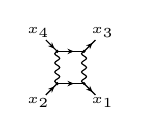
\begin{tikzpicture}[x=0.340cm, y=0.340cm, line width=0.420pt, baseline={([yshift=-0.6ex]0,0)}]
  \draw (-0.500,-0.600) -- (0.500,-0.600);
  \fill (0.119,-0.600) -- (-0.119,-0.498) -- (-0.042,-0.600) -- (-0.119,-0.702) -- cycle;
  \draw (-0.500,0.600) -- (0.500,0.600);
  \fill (0.119,0.600) -- (-0.119,0.702) -- (-0.042,0.600) -- (-0.119,0.498) -- cycle;
  \draw plot[smooth, tension=0.7] coordinates {(0.500,-0.600) (0.435,-0.557) (0.407,-0.514) (0.435,-0.471) (0.500,-0.429) (0.565,-0.386) (0.593,-0.343) (0.565,-0.300) (0.500,-0.257) (0.435,-0.214) (0.407,-0.171) (0.435,-0.129) (0.500,-0.086) (0.565,-0.043) (0.593,0.000) (0.565,0.043) (0.500,0.086) (0.435,0.129) (0.407,0.171) (0.435,0.214) (0.500,0.257) (0.565,0.300) (0.593,0.343) (0.565,0.386) (0.500,0.429) (0.435,0.471) (0.407,0.514) (0.435,0.557) (0.500,0.600)};
  \draw plot[smooth, tension=0.7] coordinates {(-0.500,-0.600) (-0.565,-0.557) (-0.593,-0.514) (-0.565,-0.471) (-0.500,-0.429) (-0.435,-0.386) (-0.407,-0.343) (-0.435,-0.300) (-0.500,-0.257) (-0.565,-0.214) (-0.593,-0.171) (-0.565,-0.129) (-0.500,-0.086) (-0.435,-0.043) (-0.407,0.000) (-0.435,0.043) (-0.500,0.086) (-0.565,0.129) (-0.593,0.171) (-0.565,0.214) (-0.500,0.257) (-0.435,0.300) (-0.407,0.343) (-0.435,0.386) (-0.500,0.429) (-0.565,0.471) (-0.593,0.514) (-0.565,0.557) (-0.500,0.600)};
  \draw (0.500,-0.600) -- (0.924,-1.024);
  \fill (0.818,-0.918) -- (0.721,-0.677) -- (0.704,-0.804) -- (0.577,-0.821) -- cycle;
  \draw (-0.500,-0.600) -- (-0.924,-1.024);
  \fill (-0.606,-0.706) -- (-0.847,-0.803) -- (-0.720,-0.820) -- (-0.703,-0.947) -- cycle;
  \draw (0.500,0.600) -- (0.924,1.024);
  \fill (0.818,0.918) -- (0.577,0.821) -- (0.704,0.804) -- (0.721,0.677) -- cycle;
  \draw (-0.500,0.600) -- (-0.924,1.024);
  \fill (-0.606,0.706) -- (-0.703,0.947) -- (-0.720,0.820) -- (-0.847,0.803) -- cycle;
  \fill (0.500,-0.600) circle (0.064);
  \fill (-0.500,-0.600) circle (0.064);
  \fill (0.500,0.600) circle (0.064);
  \fill (-0.500,0.600) circle (0.064);
  \node[font=\tiny, inner sep=0pt, anchor=135] at (0.988,-1.088) {$x_{1}$};
  \node[font=\tiny, inner sep=0pt, anchor=45] at (-0.988,-1.088) {$x_{2}$};
  \node[font=\tiny, inner sep=0pt, anchor=225] at (0.988,1.088) {$x_{3}$};
  \node[font=\tiny, inner sep=0pt, anchor=315] at (-0.988,1.088) {$x_{4}$};
\end{tikzpicture}}
